\hypertarget{probability-and-random-processes---scribing-assignment}{%
\section{Probability and Random Processes - Scribing
assignment}\label{probability-and-random-processes---scribing-assignment}}

\hypertarget{professor-prof.-lalitha-vadlamani}{%
\subsection{Professor : Prof.~Lalitha
Vadlamani}\label{professor-prof.-lalitha-vadlamani}}

\hypertarget{author-ananya-sane-l-lakshmanan}{%
\subsection{Author : Ananya Sane, L
Lakshmanan}\label{author-ananya-sane-l-lakshmanan}}

\hypertarget{lecture-9-notes}{%
\subsection{Lecture 9 notes}\label{lecture-9-notes}}

\begin{center}\rule{0.5\linewidth}{0.5pt}\end{center}

\hypertarget{key-ideas-in-lecture-9}{%
\subsection{Key Ideas in lecture 9}\label{key-ideas-in-lecture-9}}

\begin{enumerate}
\def\labelenumi{\arabic{enumi}.}
\item
  Lemmas for the CDF
\item
  Types of random variables
\end{enumerate}

\begin{center}\rule{0.5\linewidth}{0.5pt}\end{center}

\textbf{Lemma :} For any \(x \in R\)

\(P(X = x) = P(X \leq x) - P(X < x)\)

Then, by continuity of probability,

\(P(X = x) = F_X(x) - \displaystyle\lim_{\epsilon \to 0} F_X(x -\epsilon)\)

\textbf{Corollary :} \(F_X()\) is left continuous iff
\(P(X = x) = 0 \ \ \forall \ \ x \in R\)

This implies \(F_X()\) is continuous iff
\(P(X = x) = 0 \ \ \forall \ \ x \in R\)

\hypertarget{types-of-random-variables}{%
\subsubsection{Types of random
variables}\label{types-of-random-variables}}

\begin{itemize}
\item
  Continuous Random Variable
\item
  Discrete Random Variable
\item
  Mixed Random Variable

  \textbf{(Not done in class)} There is a fourth type of random variable
  called a SINGULAR random variable, that is a fundamentally different
  random variable. It is mostly only of academic interest as it does not
  have many applications. Any probability measure on the Real numbers
  can be broken down into these three fundamental components, i.e.,
  Discrete, Continuous and singular.
\end{itemize}

\hypertarget{continuous-random-variables}{%
\paragraph{Continuous Random
variables}\label{continuous-random-variables}}

A random variable X with CDF \(F_X()\) is said to be continuous if
\(F_X()\) is continuous. In the context of continuous RVs, probabilities
of intervals give useful info, as probabilities of points are always 0.

If \(F_X()\) is a differentiable function, then we can find another
function for the continuous RV, which is defined as,
\[f_X(x) = \frac{dF_X(x)}{dx}\]

which is called the \textbf{probability density function}. We can
integrate this function from \(-\infty\) to whatever value we want to
get the CDF.

So we can say that
\(P(a \leq x \leq b) = \displaystyle\int_{a}^{b}f_X(x)\cdot dx\)

And from this, if we find \(P(x \leq X \leq x + \Delta x)\) and make
\(\Delta x \to 0\), we can approximate it to a rectangle with area
\(f_X(x) \cdot \Delta x\).

\begin{figure}[''h!'']
\centering
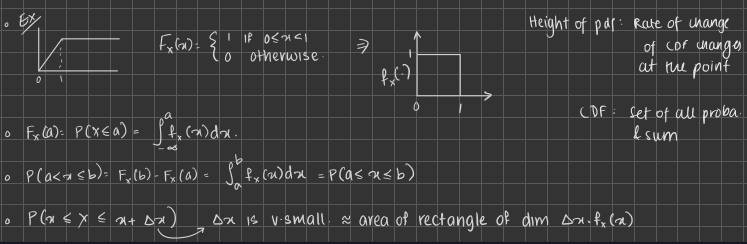
\includegraphics{Screenshot_from_2021-08-07_11-45-20.png}
\caption{Example}
\end{figure}

Properties of a PDF

\begin{itemize}
\tightlist
\item
  \(f_X(x) \geq 0\) (Because CDF is monotonically non decreasing)
\item
  \(\displaystyle\int_{-\infty}^{\infty}f_X(x)\cdot dx = 1\)
\end{itemize}

\emph{PDF by itself does not indicate any probability.}

\hypertarget{radon-nikodyn-theorem-not-done-in-class}{%
\paragraph{Radon Nikodyn theorem (Not done in
class)}\label{radon-nikodyn-theorem-not-done-in-class}}

Let X be a continuous RV. There exists a non negative measurable
function \(f_x() : R \to [0, \infty)\) such that for any B in the Borel
sigma algebra, we have

\[P_X(B) = \displaystyle\int_{B} f_x\cdot d\lambda\]

This basically means for any Borel set, we can represent its probability
law as the integral of a non negative function. As we have not done
measure theory yet, we can understand it as an integration over the real
line for our purposes. This is the basis for the equation that relates
the CDF of continuous random variables to the PDF, i.e.,

\[P_X((-\infty, x]) = F_X(x) = \displaystyle\int_{-\infty}^{x} f_X(x) dx\]

\hypertarget{discrete-random-variables}{%
\paragraph{Discrete Random Variables}\label{discrete-random-variables}}

X is said to be a discrete random variable if the range of X is either
finite or countably infinite in R.

The CDF of a discrete random variable will look like a staircase,
constant everywhere, with jumps at certain points.

Here, \(P(X = x_i) > 0\), not necessarily, but possible. CDF for this
would be

\[F_X(a) = \displaystyle\sum_{x_i \leq a} P(X = x_i)\]

Now, \(P(X = x_i) = P_X(x_i)\) for \(x_i\) in the range of X.

\(P_X()\) is called the \textbf{probability mass function}.

Properties of PMF:

\begin{itemize}
\tightlist
\item
  \(P_X(x_i) \geq 0\)
\end{itemize}

For S = range of X = \(\{x_1, x_2, ...\}\)

\begin{itemize}
\tightlist
\item
  \(\displaystyle\sum_{x_i \in S} P_X(x_i) = 1\)
\end{itemize}

\begin{center}\rule{0.5\linewidth}{0.5pt}\end{center}

\hypertarget{lecture-13-notes}{%
\subsection{Lecture 13 Notes}\label{lecture-13-notes}}

\begin{center}\rule{0.5\linewidth}{0.5pt}\end{center}

\hypertarget{key-ideas-in-lecture-13}{%
\subsection{Key ideas in lecture 13}\label{key-ideas-in-lecture-13}}

\begin{enumerate}
\def\labelenumi{\arabic{enumi}.}
\tightlist
\item
  Variance
\item
  Examples and Properties of Discrete Random Variables
\item
  Examples and Properties of Continuous Random Variables
\end{enumerate}

\begin{center}\rule{0.5\linewidth}{0.5pt}\end{center}

\hypertarget{variance-of-a-random-variable}{%
\subsection{Variance of a Random
Variable}\label{variance-of-a-random-variable}}

Variance can be understood as a quantity that represents the average
variation of a R.V about the mean. Given a R.V X, its variance is given
by

\(Var(X) = E[(X - E(X))^2] = E(X^2) - (E(X))^2\)

If X is discrete, then

\(E(X) = \mu\)

\(Var(X) = \displaystyle\displaystyle\sum_{x_i}(x_i-\mu)^2P_X(x_i)\)

If X is continuous, then

\(E(X) = \mu\)

\(Var(X) = \displaystyle\int_{-\infty}^{\infty}(x-\mu)^2f_X(x)dx\)

\hypertarget{properties-of-variance}{%
\subsubsection{Properties of Variance}\label{properties-of-variance}}

Variance is always \(\geq0\), with equality iff the random variable is
constant.

\begin{center}\rule{0.5\linewidth}{0.5pt}\end{center}

\hypertarget{examples-of-discrete-random-variables}{%
\subsection{Examples of Discrete Random
Variables}\label{examples-of-discrete-random-variables}}

\hypertarget{bernoulli-random-variables}{%
\subsubsection{1. Bernoulli Random
Variables}\label{bernoulli-random-variables}}

\begin{itemize}
\item
  Defined by

  \(P_X(x) = \begin{cases}p & for \ x=1\\1-p & for\ x=0\\0 & otherwise\end{cases}\)

  where \(0 < p < 1\).

  \begin{figure}[''h!'']
  \centering
  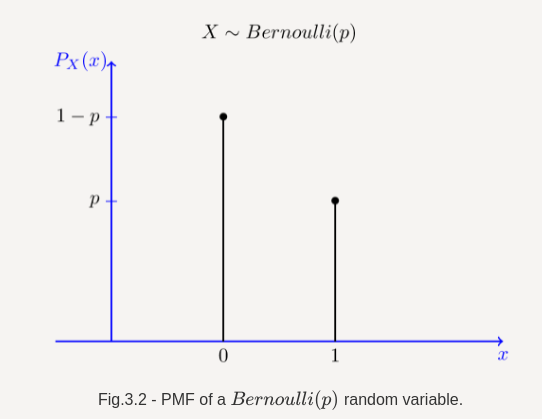
\includegraphics{Lecture 13 Notes e842fef9a3e0449fa78bac59b75dbc5c/Screenshot_from_2021-08-06_23-12-43.png}
  \caption{PMF of a Bernoulli random variable}
  \end{figure}
\item
  \(E(X) = 0(1-p) + 1(p) = p\)
\item
  \(Var(X) = (0-p)^2(1-p) + (1-p)^2(p) = p(1-p)\)
\item
  This random variable is mainly used to model random experiments that
  have two possible outcomes, which are sometimes referred to as
  ``success'' and ``failure''.
\item
  The Bernoulli random variable is also called the \textbf{Indicator
  random variable}, which tells us if a particular event has occured or
  not.
\end{itemize}

\hypertarget{binomial-random-variables}{%
\subsubsection{2. Binomial Random
Variables}\label{binomial-random-variables}}

\begin{itemize}
\item
  Experiment: Biased coin tossed \(n\) times with probability of heads
  being \(p\); outcomes mapped to \(k\) where \(k\) is the number of
  heads obtained.
\item
  This variable can be represented as the sum of \(n\) independent
  Bernoulli R.Vs.
\item
  \(P_X(x) = \begin{cases}{{n}\choose{k}} p^k(1-p)^{n-k} & for \ k=0, 1, 2, ... n\\0 & otherwise\end{cases}\)

  \begin{figure}[''h!'']
  \centering
  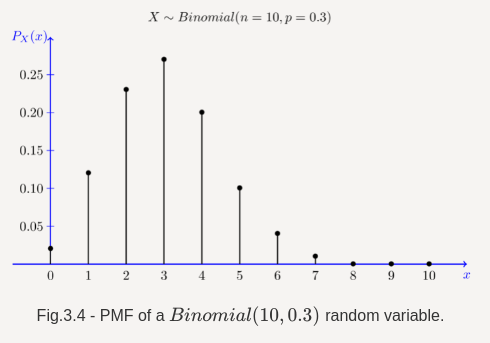
\includegraphics{Lecture 13 Notes e842fef9a3e0449fa78bac59b75dbc5c/Screenshot_from_2021-08-06_23-12-57.png}
  \caption{PMF of a binomial random variable}
  \end{figure}
\item
  \(E(X) = \displaystyle\sum_{i=0}^{n}i{n \choose i}p^i(1-p)^{n-i} = np\)
\item
  \(Var(X) =\) Sum of variances of \(n\) Bernoulli variables
  \(=nVar(X) = np(1-p)\)
\end{itemize}

\hypertarget{geometric-random-variables}{%
\subsubsection{3. Geometric Random
Variables}\label{geometric-random-variables}}

\begin{itemize}
\item
  Experiment: Toss a biased coin till a head is obtained. X is the
  position of the head.
\item
  \(P_X(k) = (1-p)^{k-1}p\)

  \begin{figure}[''h!'']
  \centering
  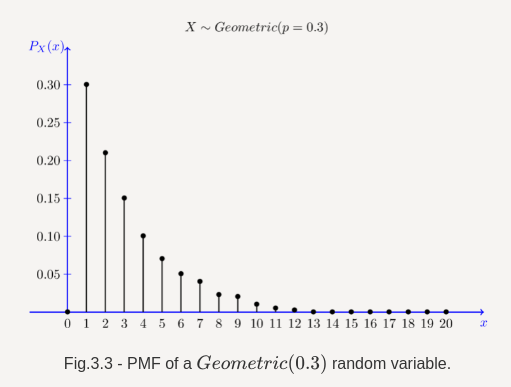
\includegraphics{Lecture 13 Notes e842fef9a3e0449fa78bac59b75dbc5c/Screenshot_from_2021-08-06_23-12-50.png}
  \caption{PMF of a geometric random variable}
  \end{figure}
\item
  \(E(X) = \displaystyle\sum_{i=0}^{n}i(1-p)^{i-1}p = 1/p\)
\item
  \(Var(X) =\) \(E(X^2) - (E(X))^2=E(X^2) -1/p^2\)

  \(E(X^2) = \displaystyle\sum_{k=1}^{\infty}k^2p(1-p)^{k-1}=(2-p)/p^2\)
\item
  \(\therefore Var(X) = (2-p-1)/p^2 = (1-p)/p^2\)
\end{itemize}

\hypertarget{poisson-random-variables}{%
\subsubsection{4. Poisson Random
Variables}\label{poisson-random-variables}}

\begin{itemize}
\item
  Used to model rare events
\item
  \(P_X(k) = \lambda^ke^{-\lambda}/k!\)

  \begin{figure}[''h!'']
  \centering
  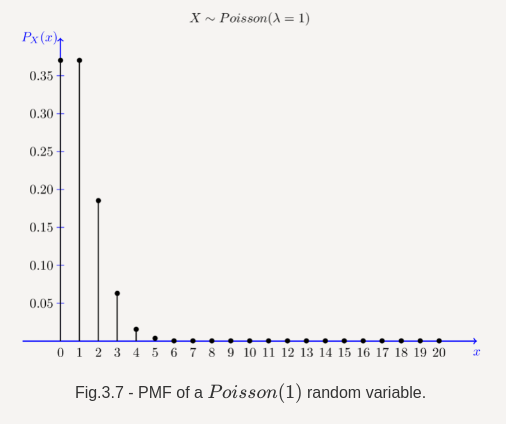
\includegraphics{Lecture 13 Notes e842fef9a3e0449fa78bac59b75dbc5c/Screenshot_from_2021-08-06_23-13-10.png}
  \caption{PMF of a poisson random variable}
  \end{figure}
\item
  \(E(X) = \lambda\)
\item
  \(Var(X) =\lambda\)
\end{itemize}

\hypertarget{pascal-random-variables-not-done-in-class}{%
\subsubsection{5. Pascal Random Variables (Not done in
class)}\label{pascal-random-variables-not-done-in-class}}

\begin{itemize}
\item
  This R.V can be understood as a generalisation of the geometric
  distribution.
\item
  Experiment: Biased coin with probability of heads being \(p\) tossed
  repeatedly until \(m\) heads are observed, \(m \in \mathcal{N}\).
\item
  As we can deduce from the above definition, a geometric variable is
  simply the case when \(m = 1\) for a Pascal random variable.
\item
  \(P_X(x) = \begin{cases}{{k-1}\choose{m-1}} p^m(1-p)^{k-m} & for \ k=m, m+1, m+2....\\0 & otherwise\end{cases}\)

  \begin{figure}[''h!'']
  \centering
  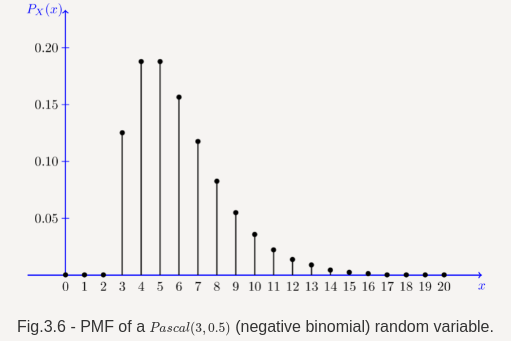
\includegraphics{../Screenshot from 2021-08-07 09-44-36.png}
  \caption{PMF of a Pascal random variable}
  \end{figure}
\item
  \(E(X) = m/p\), can be derived by expressing it as the sum of multiple
  independent geometric random variables.
\item
  \(Var(X) = m\cdot (1-p)/p^2\)
\end{itemize}

\begin{center}\rule{0.5\linewidth}{0.5pt}\end{center}

\hypertarget{examples-of-continuous-random-variables}{%
\subsection{Examples of Continuous Random
Variables}\label{examples-of-continuous-random-variables}}

\hypertarget{uniform-random-variables}{%
\subsubsection{1. Uniform Random
Variables}\label{uniform-random-variables}}

\begin{itemize}
\item
  \(f_X(x) = \begin{cases}1/(b-a) & for \ a\leq x\leq b\\0 & otherwise\end{cases}\)

  \begin{figure}[''h!'']
  \centering
  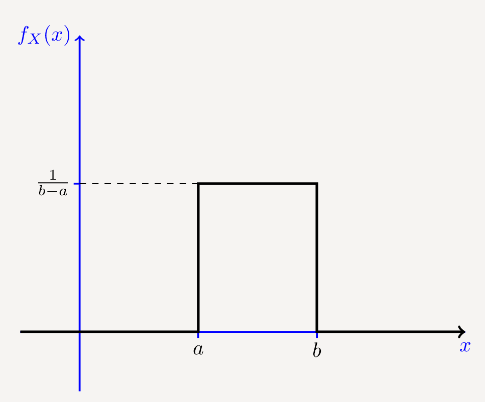
\includegraphics{Lecture 13 Notes e842fef9a3e0449fa78bac59b75dbc5c/Screenshot_from_2021-08-06_23-02-44.png}
  \caption{PDF of a uniform random variable}
  \end{figure}
\item
  \(E(X) = (a+b)/2\)
\item
  \(Var(X) = (b-a)^2/12\)
\end{itemize}

\hypertarget{exponential-random-variables}{%
\subsubsection{2. Exponential Random
Variables}\label{exponential-random-variables}}

\begin{itemize}
\item
  Used to model completion time
\item
  \(f_X(x) = \begin{cases}\lambda e^{-\lambda x} & for x\geq 0\\0 & otherwise\end{cases}\)

  \begin{figure}[''h!'']
  \centering
  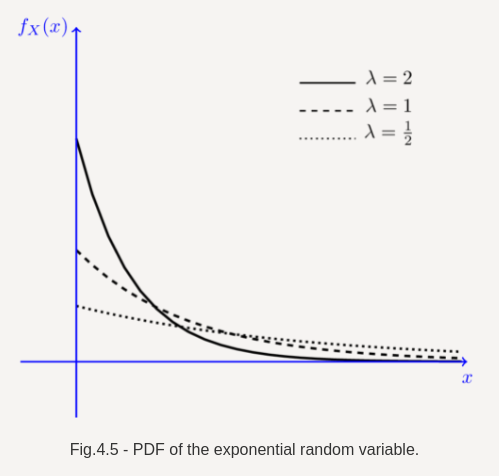
\includegraphics{Lecture 13 Notes e842fef9a3e0449fa78bac59b75dbc5c/Screenshot_from_2021-08-06_23-06-49.png}
  \caption{PDF of an exponential random variable}
  \end{figure}
\item
  \(E(X) = \displaystyle\int_{0}^{\infty}x\lambda e^{-\lambda x}dx=1/\lambda\)
\item
  \(Var(X) = 1/\lambda ^2\)
\end{itemize}

\hypertarget{gaussian-random-variables}{%
\subsubsection{3. Gaussian Random
Variables}\label{gaussian-random-variables}}

\begin{itemize}
\item
  Used to model noise. It is a sum of many independent R.V.s
\item
  \(f_X(x) = \frac{1}{\sqrt{2\pi \sigma ^2}}e^\frac{-(x-\mu)^2}{2\sigma ^2}\)

  \begin{figure}[''h!'']
  \centering
  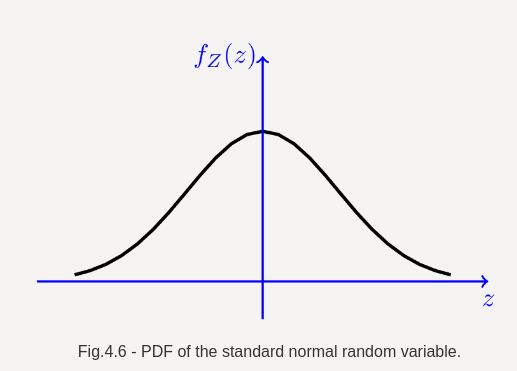
\includegraphics{Lecture 13 Notes e842fef9a3e0449fa78bac59b75dbc5c/Screenshot_from_2021-08-06_23-11-46.png}
  \caption{PDF of a standard normal random variable}
  \end{figure}
\item
  \(E(X) = \mu\)
\item
  \(Var(X) = \sigma ^2\)
\end{itemize}

\begin{center}\rule{0.5\linewidth}{0.5pt}\end{center}
